\documentclass{article}

\usepackage{graphicx}
\usepackage{tikz}
\usepackage{tikzsymbols}
\usetikzlibrary{calc,patterns,shapes.geometric}
\pagestyle{empty}
\usepackage[margin=0pt]{geometry}
\geometry{papersize={14in,12in}}

\def\centerarc[#1](#2)(#3:#4:#5){\draw[#1] ($(#2)+({#5*cos(#3)},{#5*sin(#3)})$) arc (#3:#4:#5);}

\begin{document}
	\begin{figure}
		\centering
		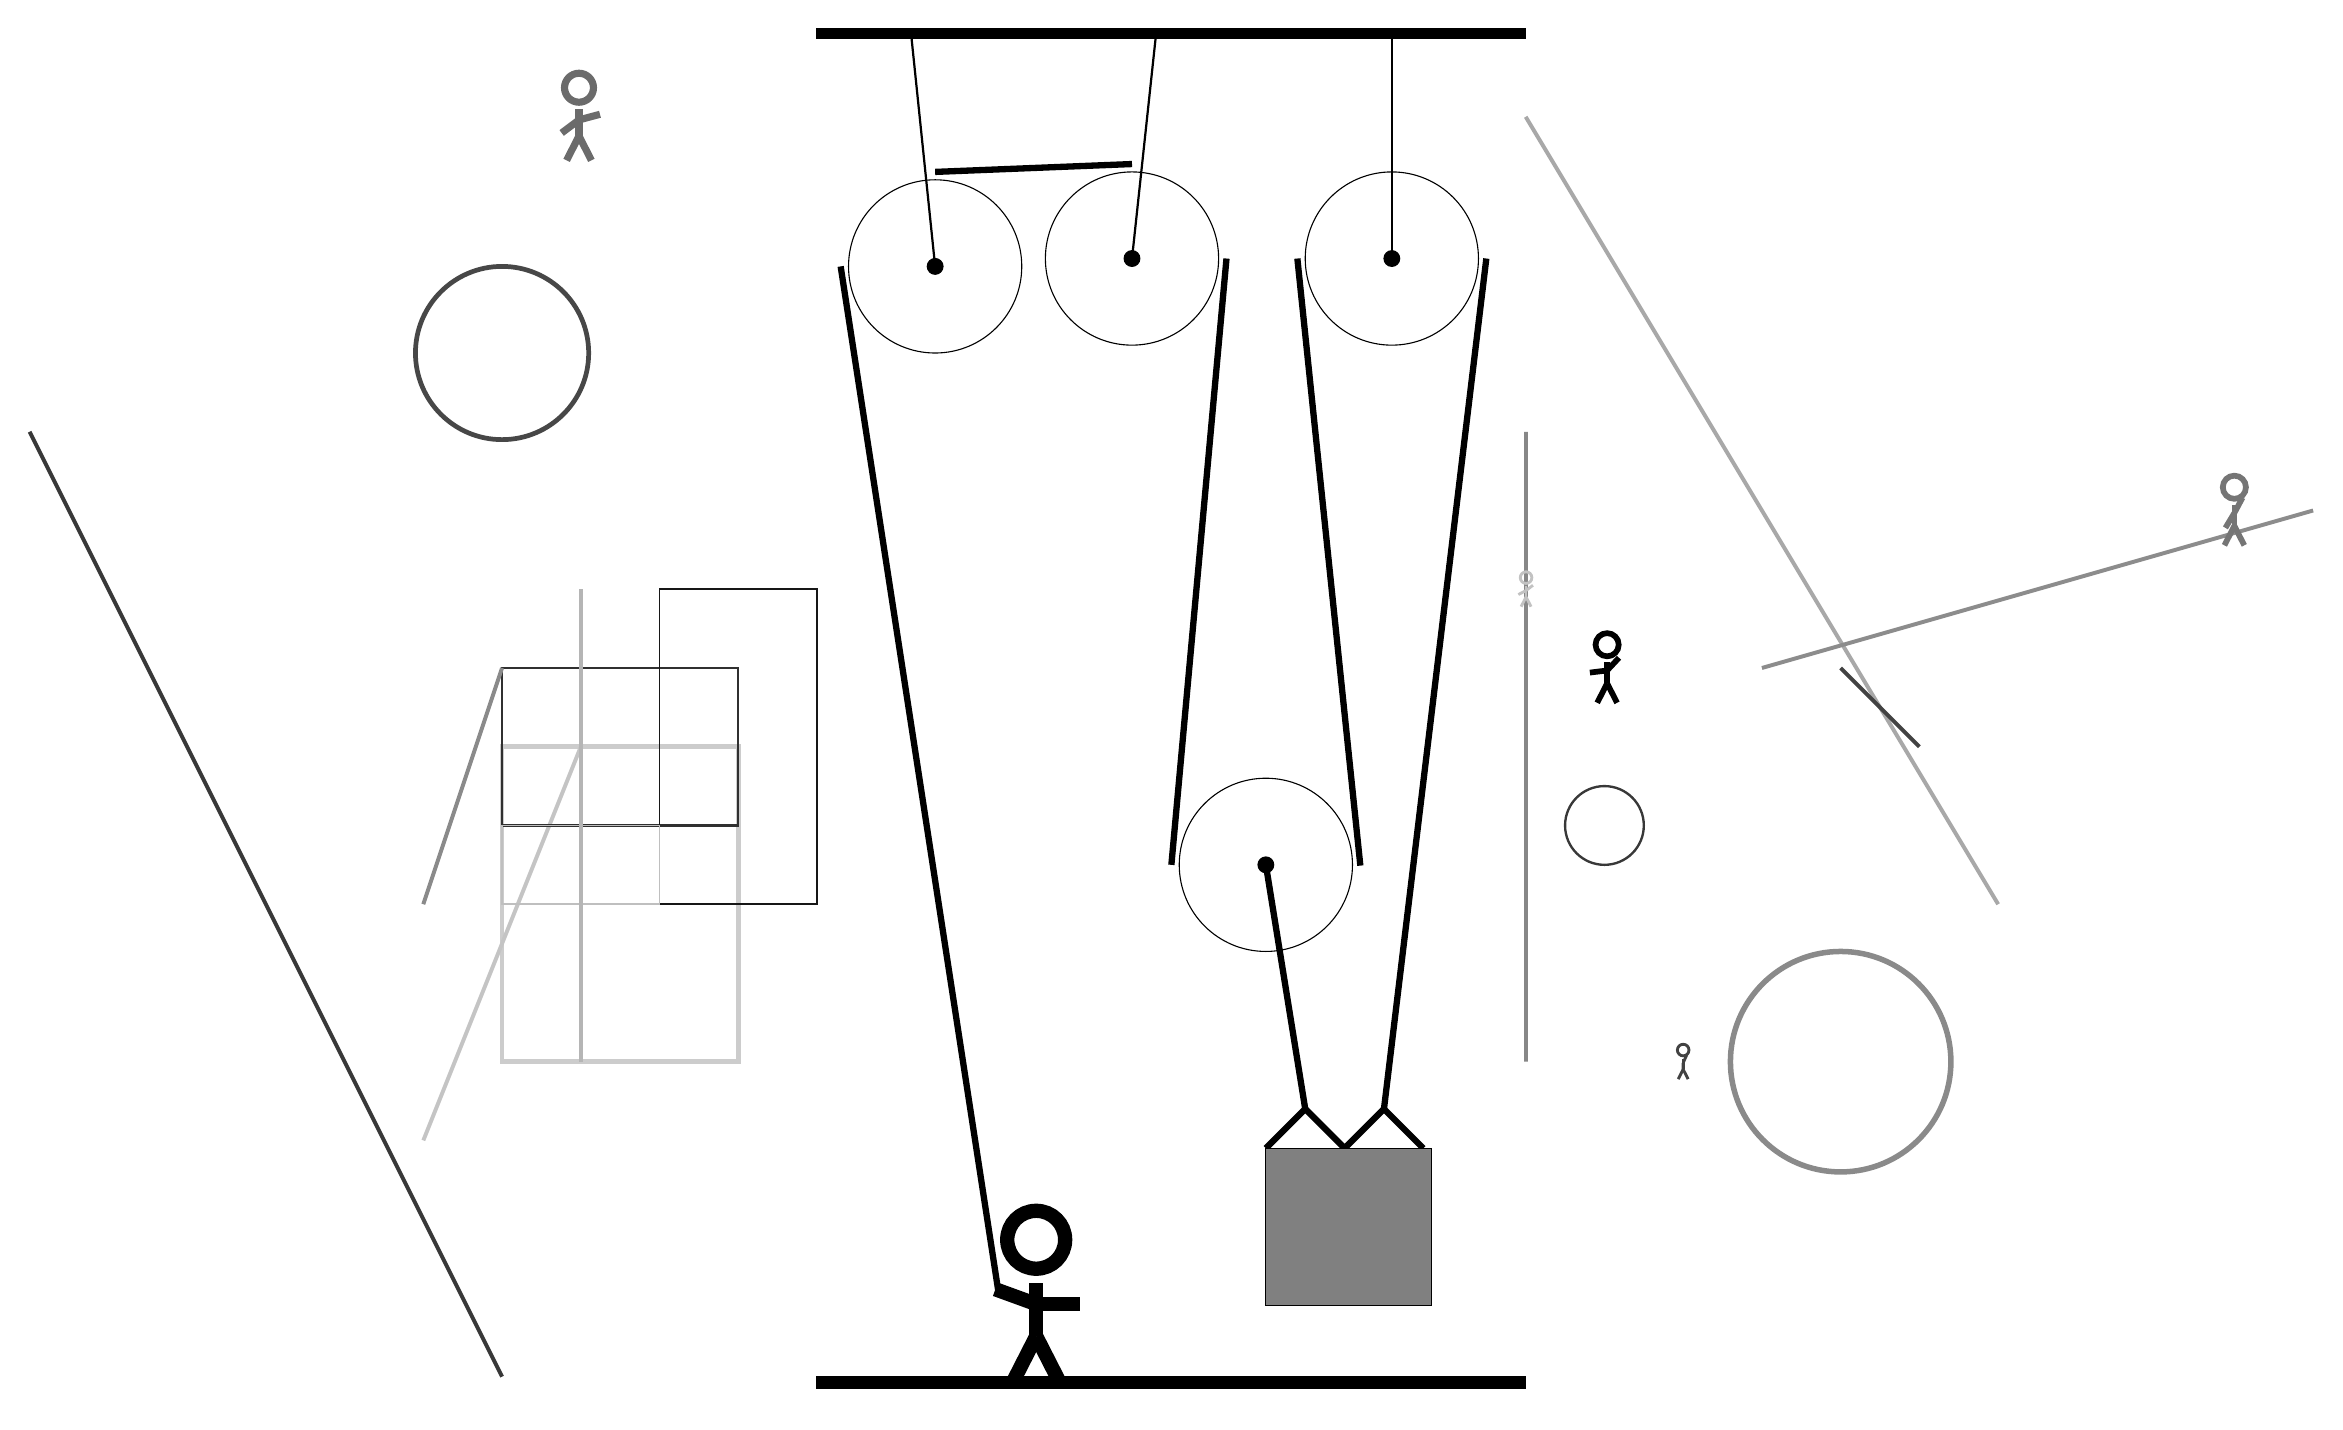
\begin{tikzpicture}
			%%%%% START %%%%%
			
			\draw[fill=black] (-3, 14) rectangle (6, 14.125);
			
			\draw (1, 11.2) circle (1.1);
			\draw[fill=black] (1, 11.2) circle (0.1);
			\draw[thick] (1, 11.2) -- (1.3, 14);
			
			\draw (4.3, 11.2) circle (1.1);
			\draw[fill=black] (4.3, 11.2) circle (0.1);
			\draw[thick] (4.3, 11.2) -- (4.3, 14);
			
			\draw (2.7, 3.5) circle (1.1);
			\draw[fill=black] (2.7, 3.5) circle (0.1);
			
			\draw[line width=0.8mm]  (2.7, -0.1) -- (3.2, 0.4) -- (3.7, -0.1) -- (4.2, 0.4) -- (4.7, -0.1);
			\draw[fill=black!50] (2.7, -0.1) rectangle (4.8, -2.1);
			
			\draw[line width=0.6mm, color=black!20] (-4, 5) rectangle (-7, 1);
			
			\draw[line width=0.5mm, color=black!23](-6, 5) -- (-8, 0);
			\draw[line width=0.3mm, color=black!81] (-4, 6) rectangle (-7, 4);
			\draw[line width=0.5mm, color=black!47] (6, 1) rectangle (6, 9);
			
			\draw[line width=0.5mm, color=black!46](-7, 6) -- (-8, 3);
			\draw [line width=0.3mm, color=black!78](7, 4) circle (0.5);
			\draw[line width=0.5mm, color=black!34](6, 13) -- (12, 3);
			\node[line width=0.2mm, color=black!100] at (7, 6) {\Strichmaxerl[4][7][47]};
			\draw[line width=0.2mm, color=black!91] (-5, 3) rectangle (-3, 7);
			\draw[line width=0.5mm, color=black!74](10, 6) -- (11, 5);
			\draw [line width=0.7mm, color=black!46](10, 1) circle (1.4);
			\draw[line width=0.5mm, color=black!45](9, 6) -- (16, 8);
			\draw[line width=0.5mm, color=black!78](-7, -3) -- (-13, 9);
			
			\node[line width=0.7mm, color=black!58] at (-6, 13) {\Strichmaxerl[5][37][15]};
			\node[line width=0.6mm, color=black!24] at (6, 7) {\Strichmaxerl[2][28][37]};
			\draw[line width=0.2mm, color=black!25] (-5, 4) rectangle (-7, 3);
			
			\draw[line width=0.5mm, color=black!29](-6, 1) -- (-6, 7);
			\node[line width=0.3mm, color=black!74] at (8, 1) {\Strichmaxerl[2][89][66]};
			\draw [line width=0.6mm, color=black!72](-7, 10) circle (1.1);
			\node[line width=0.5mm, color=black!54] at (15, 8) {\Strichmaxerl[4][59][62]};
			
			\draw (-1.5, 11.1) circle (1.1);
			\draw[fill=black] (-1.5, 11.1) circle (0.1);
			\draw[thick] (-1.5, 11.1) -- (-1.8, 14);
			
			\draw[line width=0.8mm](-0.7, -1.9) --  (-2.7, 11.1);
			\centerarc[line width=0.8mm](-1.5, 11.1)(90:180:1.2000000000000002);
			\draw[line width=0.8mm](-1.5, 12.3) -- (1, 12.4);
			\centerarc[line width=0.8mm](1, 11.2)(0:90:1.2000000000000002);
			\draw[line width=0.8mm](2.2, 11.2) -- (1.5, 3.5);
			\centerarc[line width=0.8mm](2.7, 3.5)(180:370:1.2000000000000002);
			\draw[line width=0.8mm] (3.9, 3.49) -- (3.1, 11.2);
			\centerarc[line width=0.8mm](4.3, 11.2)(0:180:1.2000000000000002);
			\draw[line width=0.8mm](4.2, 0.4) -- (5.5, 11.2);
			\draw[line width=0.8mm] (3.2, 0.4) -- (2.7, 3.5);
			
			\node at (-0.2, -2) {\Strichmaxerl[10][-20][0]};
			
			\draw[fill=black] (-3, -3) rectangle (6, -3.15);
			
			%%%%% END %%%%%
		\end{tikzpicture}
	\end{figure}	
\end{document}